\section{Introduction}
\label{sec:introduction}
\IEEEPARstart{T}{iny Tapeout} is a multi project chip platform that makes it easier and cheaper to get application specific integrated circuit (ASIC) designs manufactured.

Open source tools and process design kits (PDK~\cite{pdk}) are used so no licenses or non disclosure agreement (NDAs) are required. As the tools run on remote cloud servers no software needs to be installed locally on the user's machine. As long as the template structure is followed, however, Tiny Tapeout does support the use of proprietary tools.

Each Tiny Tapeout ASIC production run sees around 400 open source designs multiplexed to 24 general purpose input/output (GPIO) pins. After manufacture the resulting chip is mounted to a demonstration board for ease of testing. Each chip contains a copy of every design, which can be selected and tested in turn.

At the same time each participant submits documentation for their design, which used to create a printable datasheet~\cite{datasheet} along with an online project index at TinyTapeout.com/runs/~\cite{tinytapeoutruns}. The datasheet helps participants explore other designs on the chip in addition to their own.

By separating the cost of area on a silicon wafer and the finished physical chip, the Tiny Tapeout participant group is able to share the cost of chip packaging and circuit board manufacture while still being able to test and measure all the designs on the chip. For use in educational settings it is possible for multiple students to submit individual designs while sharing the finished chips and circuit boards, reducing the cost still further.

Each Tiny Tapeout tile (Fig.~\ref{fig:render_cells_in_use}) is approximately $160 \times \qty{100}{\micro\meter\squared}$. This provides enough room for around 1000 logic gates when built upon the SkyWater 130nm open source PDK. Multiple tiles can be interconnected to enable larger designs, while analog and mixed signal support is on the roadmap for the next shuttle.

Community engagement in Tiny Tapeout has been strong, with 756 designs submitted over the first five shuttles. A curated selection of projects is provided in section~\ref{sec:silicon_showcase}.
An online chat server for participants has 1000 members with 1600 subscribers to the project's mailing list. Individuals submitting designs to Tiny Tapeout tend to self identify as hobbyists, students, and teachers, as shown in Fig.~\ref{fig:TT04_submitters}.

The first~\cite{firstshuttle} Tiny Tapeout production run, which was provided as a free and experimental effort with a total of 152 designs, was submitted to the seventh Google-sponsored~\cite{googlesponsored} lottery based multi project wafer (MPW) shuttle in September 2022.
The next four shuttles combined a total of 582 designs, all sponsored by and manufactured through the Efabless~\cite{efabless} chipIgnite MPW service. Table~\ref{tab:tinytapeout} shows a summary of all Tiny Tapeout shuttle runs to date.

The rest of this paper will detail the Tiny Tapeout design flow, multiplexer evolution, circuit board design, the results of post production silicon testing, and the project's next steps.

\begin{table*}[!t]
\centering
\caption{Tiny Tapeout shuttle summary}
\label{tab:tinytapeout}
\begin{tabularx}{\textwidth}{@{}l *{9}{X}@{}}
\toprule
\textbf{Run} & \textbf{Launched} & \textbf{Shuttle} & \textbf{Designs} & \textbf{Delivery date} & \textbf{Architecture} & \textbf{Number of IOs} & \textbf{IO bandwidth} & \textbf{Analog support} \\
\midrule
TT01 & 2022-08-17  & MPW7  & 152 & n/a        & Scan chain                & 16 & \qty{5}{\kHz}    & no  \\
TT02 & 2022-11-09  & 2211Q & 165 & 2024-01-30 & Scan chain                & 16 & \qty{5}{\kHz}    & no  \\
TT03 & 2023-03-01  & 2304C & 249 & 2024-02-28 & Scan chain inverted clock & 16 & \qty{10}{\kHz}    & no  \\
TT04 & 2023-07-01  & 2309  & 143 & 2024-04-15 & Mux                       & 26 & \qty{50}{\MHz}   & no  \\
TT05 & 2023-09-11  & 2311  & 174 & 2024-05-12 & Split Mux                 & 26 & \qty{50}{\MHz}   & no  \\
TT06 & 2024-02-01  & 2404  & TBD & 2024-11-30 & Split Mux                 & 38 & \qty{50}{\MHz}   & yes \\
\bottomrule
\end{tabularx}
\end{table*}

\begin{figure}[!t]
\centering
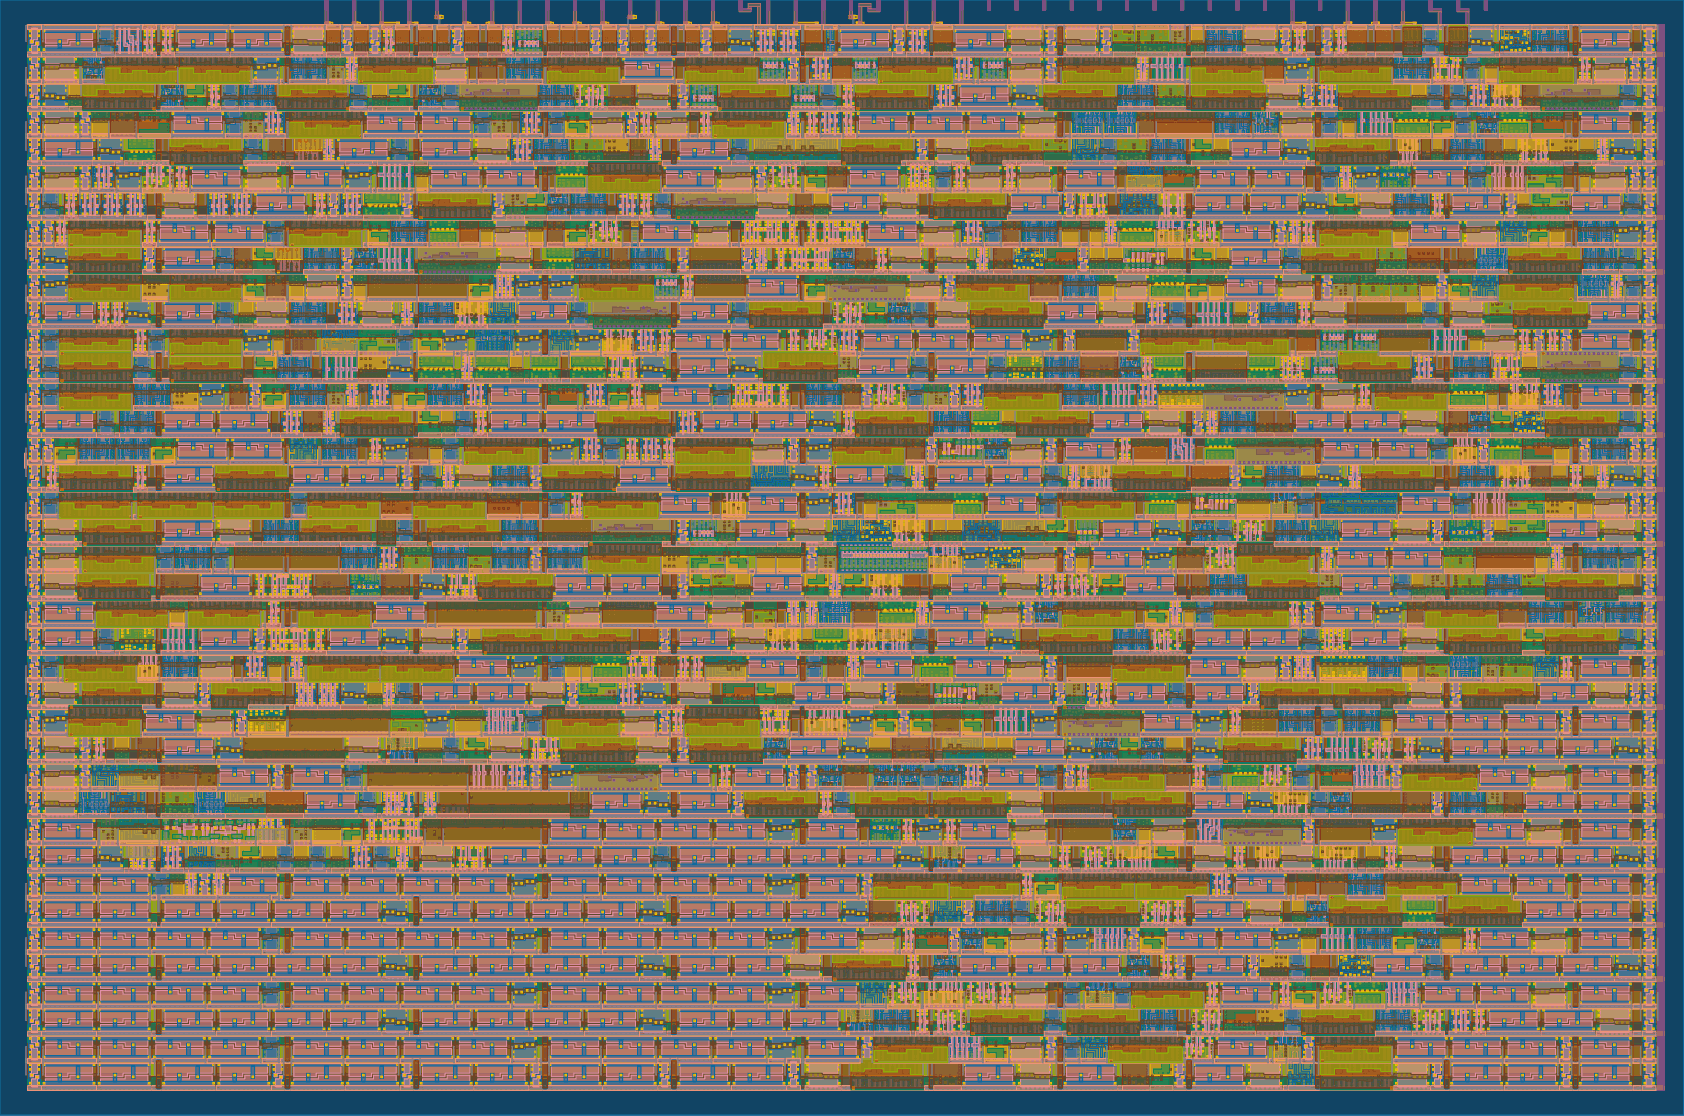
\includegraphics[width=\columnwidth]{./Figs/gh action gds layout.png}
\caption{A 2-D render of a single Tiny Tapeout tile.}
\label{fig:render_cells_in_use}
\end{figure}

\begin{figure}[!t]
\centering
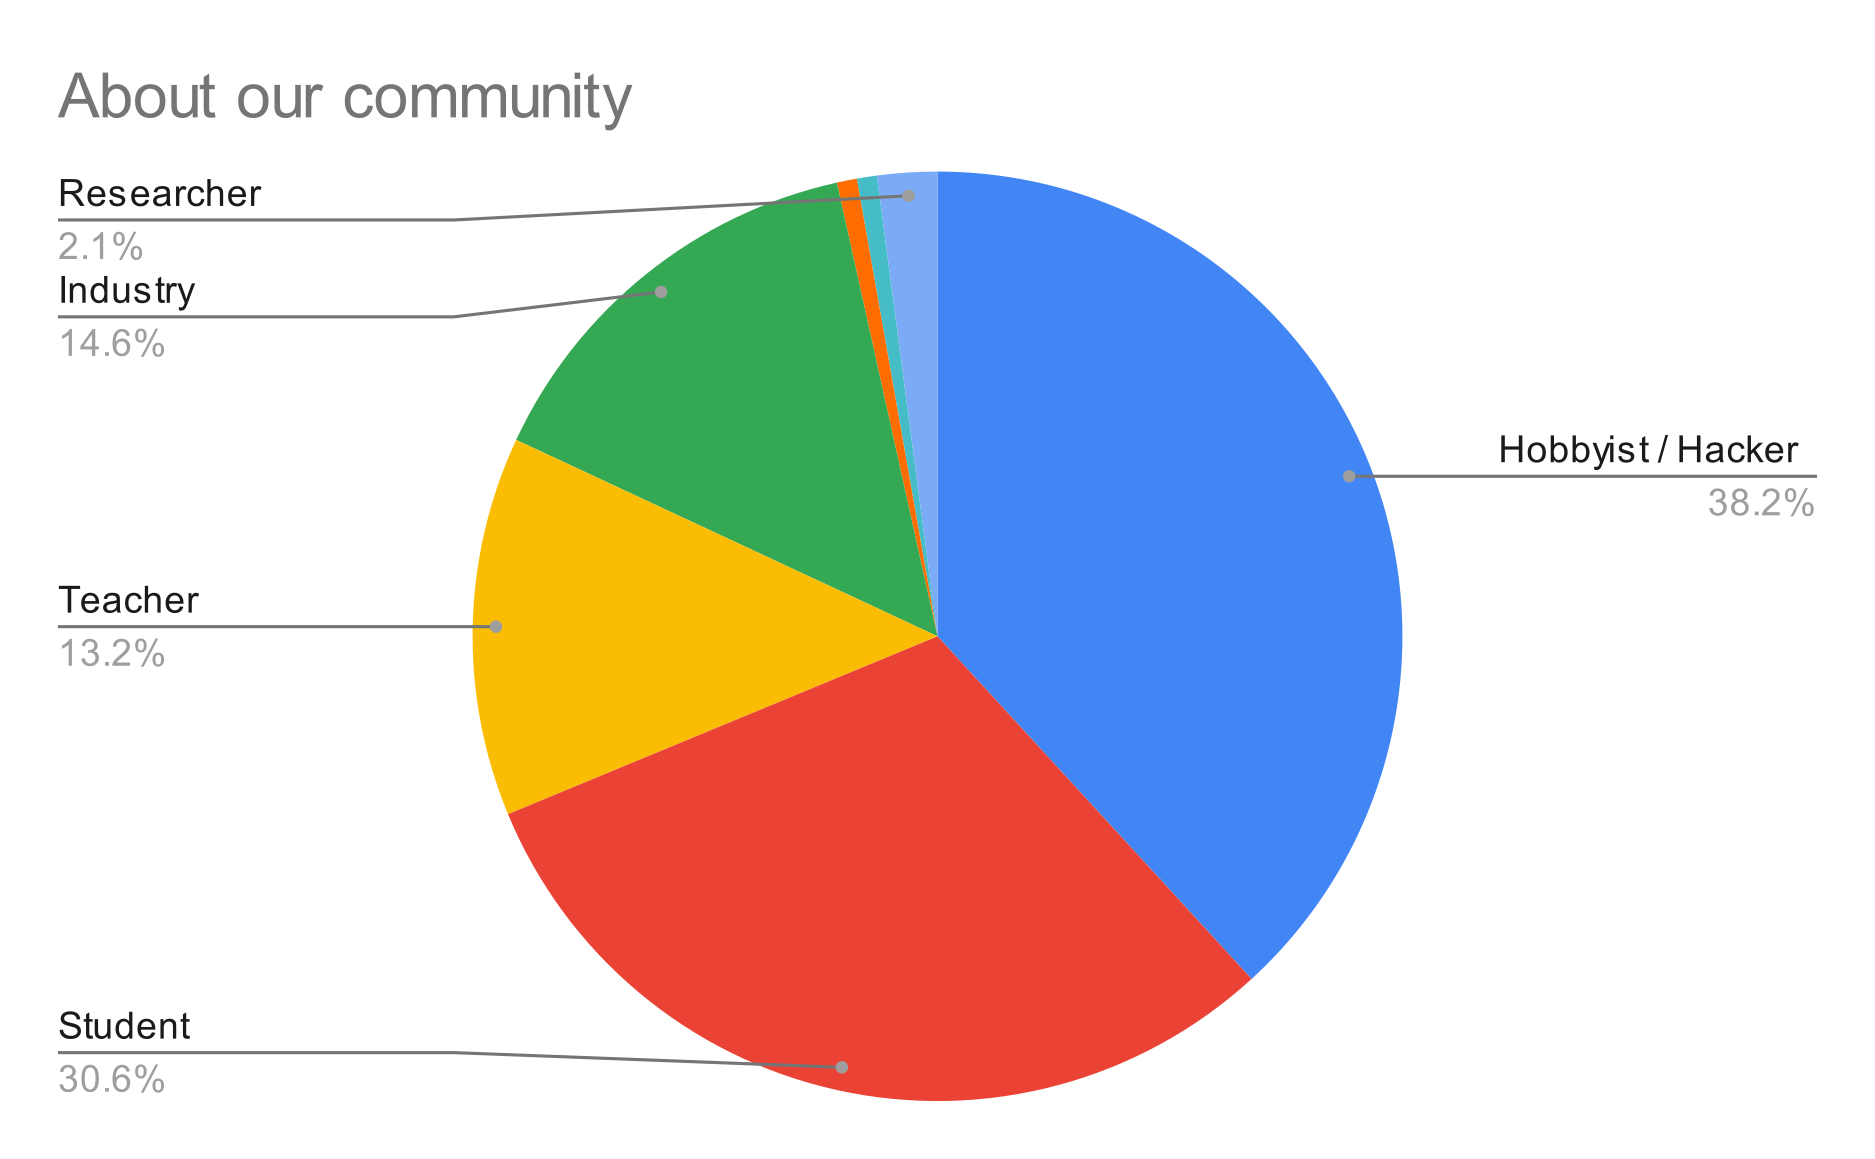
\includegraphics[width=\columnwidth]{./Figs/about our community pie chart.png}
\caption{Tiny Tapeout 4 participant self identification.}
\label{fig:TT04_submitters}
\end{figure}
